% ══════════════════════════════════════════════════════════════════════════
% Pluribus in this codebase — from the idea to the code (trainer/pluribus)
% Companion to modern_poker_ai_tutorial.pdf (its Pluribus section is the
% "theory" side; this document maps that theory onto the implementation).
% Build:  pdflatex pluribus_implementation.tex   (run twice for refs/toc)
% ══════════════════════════════════════════════════════════════════════════
\documentclass[11pt,a4paper]{article}

\usepackage[utf8]{inputenc}
\usepackage[T1]{fontenc}
\usepackage{lmodern}
\usepackage[margin=2.2cm]{geometry}
\usepackage{amsmath,amssymb}
\usepackage[dvipsnames]{xcolor}
\usepackage{tikz}
\usetikzlibrary{arrows.meta,positioning,shapes.geometric,calc,fit,backgrounds}
\usepackage{listings}
\usepackage{tcolorbox}
\usepackage{booktabs}
\usepackage{enumitem}
\usepackage[colorlinks=true,linkcolor=MidnightBlue,urlcolor=MidnightBlue,citecolor=MidnightBlue]{hyperref}

% ─── Palette (same as the tutorials) ────────────────────────────────────────
\definecolor{accent}{RGB}{25,55,110}
\definecolor{heroG}{RGB}{20,110,60}
\definecolor{villR}{RGB}{160,40,40}
\definecolor{memO}{RGB}{190,110,10}
\definecolor{codebg}{RGB}{246,247,249}
\definecolor{codekw}{RGB}{0,80,160}
\definecolor{codecomment}{RGB}{100,120,100}
\definecolor{codestr}{RGB}{150,60,20}

\lstdefinestyle{py}{
  language=Python,
  basicstyle=\ttfamily\small,
  keywordstyle=\color{codekw}\bfseries,
  commentstyle=\color{codecomment}\itshape,
  stringstyle=\color{codestr},
  backgroundcolor=\color{codebg},
  frame=single, rulecolor=\color{black!25},
  framesep=6pt, xleftmargin=10pt, xrightmargin=4pt,
  showstringspaces=false,
  columns=fullflexible, keepspaces=true,
  breaklines=true,
  literate={σ}{$\sigma$}1 {β}{$\beta$}1 {θ}{$\theta$}1 {≈}{$\approx$}1
           {×}{$\times$}1 {→}{$\rightarrow$}1 {Σ}{$\Sigma$}1 {·}{$\cdot$}1
           {Δ}{$\Delta$}1 {≤}{$\leq$}1 {≥}{$\geq$}1
}

\newtcolorbox{intuition}{
  colback=blue!4, colframe=accent, boxrule=0.8pt, arc=2mm,
  title=\textbf{Intuition}, fonttitle=\color{white},
  left=6pt, right=6pt, top=4pt, bottom=4pt}
\newtcolorbox{trap}{
  colback=red!4, colframe=villR, boxrule=0.8pt, arc=2mm,
  title=\textbf{Watch out}, fonttitle=\color{white},
  left=6pt, right=6pt, top=4pt, bottom=4pt}
\newtcolorbox{defbox}{
  colback=black!3, colframe=black!50, boxrule=0.6pt, arc=2mm,
  left=6pt, right=6pt, top=4pt, bottom=4pt}

\setlength{\parskip}{4pt}
\setlength{\parindent}{0pt}
\newcommand{\file}[1]{\textcolor{accent}{\texttt{#1}}}
\newcommand{\fn}[1]{\texttt{#1}}

\begin{document}

% ─── Title ──────────────────────────────────────────────────────────────────
\begin{center}
  {\Huge\bfseries Pluribus, in this codebase}\\[2mm]
  {\large from the idea to the code --- a guided tour of \texttt{trainer/pluribus}}\\[3mm]
  {\normalsize A tabular blueprint (\textbf{no neural network}) plus depth-limited
   search, implemented for heads-up no-limit hold'em}\\[2mm]
  {\small Companion to \texttt{docs/modern\_poker\_ai\_tutorial.pdf} --- that document
   is the \emph{theory} (its Pluribus section); this one is the \emph{map from
   theory to code}.}
\end{center}
\vspace{2mm}
\hrule
\vspace{3mm}

\begin{intuition}
Pluribus's one idea (tutorial, §Pluribus): a coarse offline \textbf{blueprint}
strategy --- computed by \textbf{Linear MCCFR} over an \emph{abstracted} game and
stored in \textbf{regret tables}, with \emph{no neural network} --- plus cheap
\emph{depth-limited} online \textbf{re-solving} is enough to play superhuman poker.
It famously trained on a \textbf{64-core CPU server, no GPU}: the scarce resource
is RAM for the tables, not FLOPs. This codebase implements that \emph{method} over
the project's heads-up engine (the engine is 2-player; ReBeL was ported the same
way). Every Pluribus concept below is named with the file and function that
realizes it.
\end{intuition}

\tableofcontents
\vspace{3mm}\hrule

% ════════════════════════════════════════════════════════════════════════════
\section{High-level view: the module map}
% ════════════════════════════════════════════════════════════════════════════

\file{trainer/pluribus/} is pure Python. It reuses the pybind engine
(\texttt{pokertrainer\_engine}) to enumerate legal bets and evaluate hands, and
reuses \file{trainer/rebel\_py} for the \emph{search} primitives (the 1326-combo
hand index, showdown values, the vectorized CFR-D subgame solver and the
best-response gate) --- ReBeL and Pluribus share the search; what differs is that
Pluribus's blueprint is \textbf{tables, not a net}, and its leaves are valued by
\textbf{continuation strategies}, not a value network.

\begin{center}
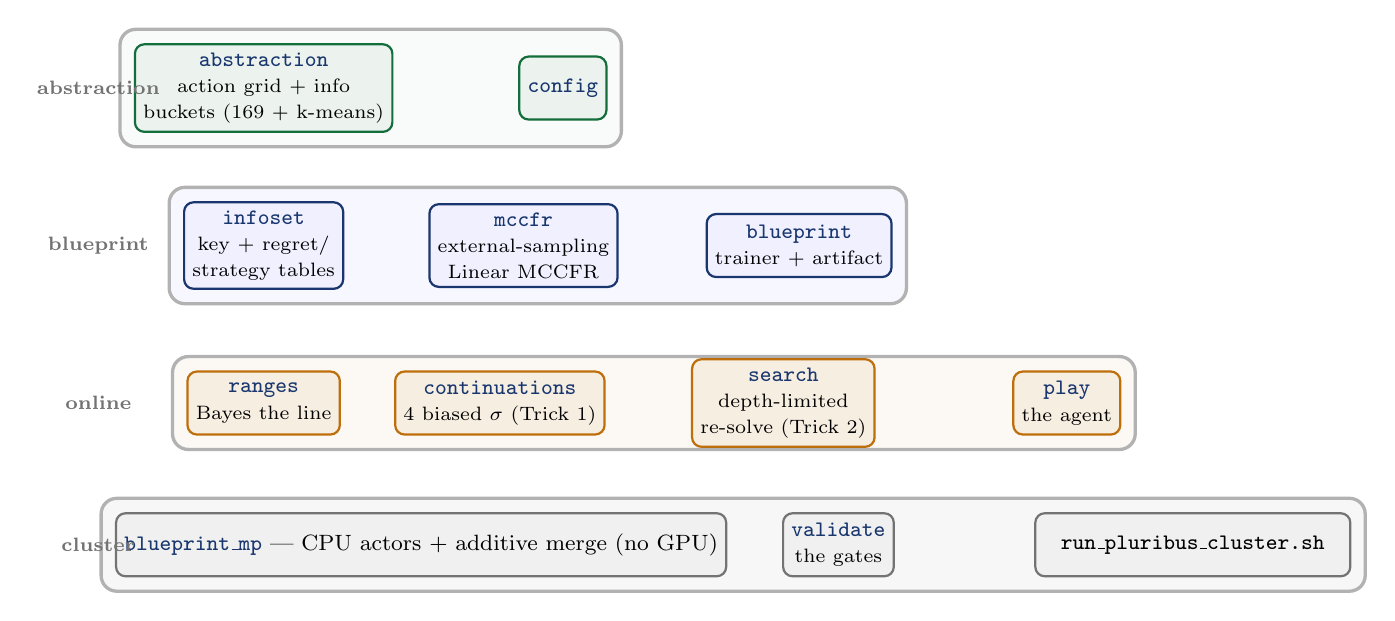
\begin{tikzpicture}[font=\footnotesize, >={Stealth[length=2mm]},
  box/.style={rectangle, rounded corners=1.2mm, draw, thick, align=center,
              minimum height=8mm, inner sep=3pt, fill=white},
  lay/.style={rectangle, rounded corners=2mm, draw=black!30, very thick,
              inner sep=5pt},
  lbl/.style={font=\scriptsize\bfseries, text=black!55}]

% Layer 1: abstraction
\node[box, fill=heroG!8, draw=heroG] (ab) at (0.4,0)
     {\file{abstraction}\\ \scriptsize action grid + info\\ \scriptsize buckets (169 + k-means)};
\node[box, fill=heroG!8, draw=heroG] (cf) at (4.2,0) {\file{config}};
\node[lbl] at (-1.7,0) {abstraction};

% Layer 2: blueprint
\node[box, fill=blue!6, draw=accent] (is) at (0.4,-2.0) {\file{infoset}\\ \scriptsize key + regret/\\ \scriptsize strategy tables};
\node[box, fill=blue!6, draw=accent] (mc) at (3.7,-2.0){\file{mccfr}\\ \scriptsize external-sampling\\ \scriptsize Linear MCCFR};
\node[box, fill=blue!6, draw=accent] (bp) at (7.2,-2.0){\file{blueprint}\\ \scriptsize trainer + artifact};
\node[lbl] at (-1.7,-2.0) {blueprint};

% Layer 3: online search
\node[box, fill=memO!12, draw=memO] (rg) at (0.4,-4.0) {\file{ranges}\\ \scriptsize Bayes the line};
\node[box, fill=memO!12, draw=memO] (co) at (3.4,-4.0){\file{continuations}\\ \scriptsize 4 biased $\sigma$ (Trick 1)};
\node[box, fill=memO!12, draw=memO] (se) at (7.0,-4.0){\file{search}\\ \scriptsize depth-limited\\ \scriptsize re-solve (Trick 2)};
\node[box, fill=memO!12, draw=memO] (pl) at (10.6,-4.0){\file{play}\\ \scriptsize the agent};
\node[lbl] at (-1.7,-4.0) {online};

% Layer 4: cluster
\node[box, fill=black!6, draw=black!55, minimum width=46mm] (mp) at (2.4,-5.8)
     {\file{blueprint\_mp} --- CPU actors + additive merge (no GPU)};
\node[box, fill=black!6, draw=black!55] (vl) at (7.7,-5.8) {\file{validate}\\ \scriptsize the gates};
\node[box, fill=black!6, draw=black!55, minimum width=40mm] (sc) at (12.2,-5.8)
     {\texttt{run\_pluribus\_cluster.sh}};
\node[lbl] at (-1.7,-5.8) {cluster};

\begin{scope}[on background layer]
  \node[lay, fit=(ab)(cf), fill=heroG!3] {};
  \node[lay, fit=(is)(bp), fill=blue!3] {};
  \node[lay, fit=(rg)(pl), fill=memO!4] {};
  \node[lay, fit=(mp)(sc), fill=black!3] {};
\end{scope}
\end{tikzpicture}
\end{center}

\paragraph{The phases (how it was built and validated).}
\begin{center}\small
\begin{tabular}{@{}lll@{}}
\toprule
Phase & What & Gate (proof it is correct) \\
\midrule
1 & tabular Linear-MCCFR blueprint $+$ abstraction & 10bb push/fold $=$ Nash oracle \\
  &  (no search) & (SB jam 58.0 vs 58.1\%, BB call 37.6 vs 37.3\%) \\
2 & depth-limited online re-solving & river re-solve $\to 0.002$ bb/hand exploit. \\
  &  (Tricks 1 \& 2 $+$ nested) & (whole 1326-hand range) \\
3 & cluster blueprint trainer & 64-core actor pool; additive table merge; \\
  &  (CPU actors, no GPU) & checkpoints round-trip \\
\bottomrule
\end{tabular}
\end{center}

\begin{intuition}
\textbf{What is Pluribus's, and what is shared with ReBeL?} The blueprint half
(\file{abstraction}, \file{infoset}, \file{mccfr}, \file{blueprint}) is pure
Pluribus and has no ReBeL analogue --- it is the ``no neural network'' branch.
The search half reuses \file{rebel\_py}'s vectorized CFR-D solver and
exploitability gate (the math of solving a public subgame over the 1326-combo
range is identical); Pluribus only swaps the value-net leaf for a
continuation-strategy leaf (Trick 1) and feeds it Bayes ranges built from the
\emph{tabular} blueprint.
\end{intuition}

% ════════════════════════════════════════════════════════════════════════════
\section{Information \& action abstraction (\file{abstraction.py})}
% ════════════════════════════════════════════════════════════════════════════

Two abstractions shrink $10^{161}$ situations to a table that fits in RAM.

\paragraph{Action abstraction.} \fn{ActionAbstraction.actions(state, legal)}
restricts the engine's 11 actions to a small grid. The \texttt{"pushfold"} preset
is the Phase-1 gate (preflop jam/fold for the opener, call/fold facing an all-in
--- exactly the game the Nash oracle solves); \texttt{"discrete"} is a per-street
pot-fraction grid that always force-includes fold/call/all-in so the tree closes.
Betting is hole-independent, so this is a function of the public state only.

\paragraph{Information abstraction.} \fn{InfoAbstraction.bucket\_cards(street,
board, c0, c1)} maps a situation to a bucket id.

\begin{itemize}[leftmargin=1.4em, itemsep=2pt]
\item \textbf{Preflop is lossless}: the 169 strategic classes
  (\texttt{evaluate.preflop\_equity.class\_of}), shared with the push/fold oracle.
\item \textbf{Postflop is k-means on equity-distribution histograms}. A hand on a
  board is described by the \emph{shape} of its equity across runouts --- so a
  made hand (mass near 1) and a draw (bimodal) separate even at equal raw equity.
  Centroids are learned on a board \emph{sample} (\fn{learn\_street\_buckets});
  every situation is assigned to its nearest centroid at run time, cached.
\end{itemize}

\begin{center}
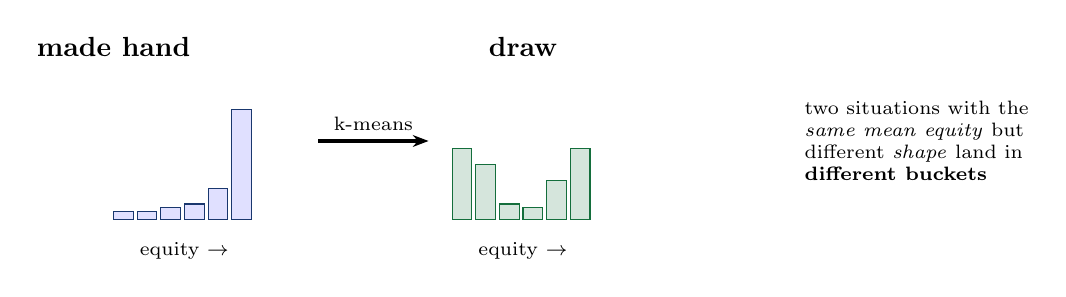
\begin{tikzpicture}[font=\scriptsize, >={Stealth[length=2mm]},
  bar/.style={draw=accent, fill=blue!12}]
  % made hand histogram
  \node[font=\bfseries] at (0,2.2) {made hand};
  \foreach \x/\h in {0/0.1,0.3/0.1,0.6/0.15,0.9/0.2,1.2/0.4,1.5/1.4} {
     \draw[bar] (\x,0) rectangle (\x+0.25,\h);}
  \node at (0.9,-0.4) {equity $\to$};
  % draw histogram (bimodal)
  \node[font=\bfseries] at (5.2,2.2) {draw};
  \foreach \x/\h in {0/0.9,0.3/0.7,0.6/0.2,0.9/0.15,1.2/0.5,1.5/0.9} {
     \draw[bar, fill=heroG!18, draw=heroG] (\x+4.3,0) rectangle (\x+4.55,\h);}
  \node at (5.2,-0.4) {equity $\to$};
  \draw[->, very thick] (2.6,1.0) -- node[above]{k-means} (4.0,1.0);
  \node[align=left] at (10.2,1.0)
    {two situations with the\\ \emph{same mean equity} but\\ different \emph{shape}
     land in\\ \textbf{different buckets}};
\end{tikzpicture}
\end{center}

\begin{trap}
The Phase-1 push/fold gate is \emph{preflop-only}, so it never touches the k-means
path. A full ``discrete'' postflop game needs a learned bucket cache; without one,
\fn{bucket\_cards} falls back to the (coarse) preflop class and prints a warning.
Building the real per-street buckets is the offline precompute that the cluster
run owns.
\end{trap}

% ════════════════════════════════════════════════════════════════════════════
\section{The blueprint: tabular Linear MCCFR (\file{infoset.py}, \file{mccfr.py}, \file{blueprint.py})}
% ════════════════════════════════════════════════════════════════════════════

\begin{defbox}
\textbf{Abstract infoset key} (\fn{infoset\_key}): \texttt{(street, to\_act,
bucket, history\_token)}, where the history token is the chronological tuple of
engine \texttt{ActionType} ints applied so far. Two situations mapping to the same
key share a strategy --- that sharing is what makes the table small. Regret and
strategy-sum are plain dicts \texttt{key $\to$ ndarray[11]} (\fn{Tables}),
\textbf{sparse} and \textbf{additive} (the property the cluster merge needs).
\end{defbox}

\fn{mccfr.traverse} is one external-sampling Linear-MCCFR traversal --- the same
scheme as the repo's Deep CFR (\texttt{cfr\_coro}), but writing to tables instead
of neural-net buffers:

\begin{lstlisting}[style=py, caption={\file{mccfr.py} --- the traversal. $\sigma$ is read by regret matching on the stored regrets; it is accumulated for the average strategy ONLY at opponent nodes (Brown 2019, Alg.~1), where sampling visits $\propto$ the opponent's own reach.}]
def traverse(env, traverser, weight, tables, abstraction, rng, allin_samples=0):
    if env.is_terminal():
        # variance reduction: value an all-in showdown by Monte-Carlo equity
        # over K runouts, not the single board the engine happened to deal.
        if allin_samples and both_all_in(env): return allin_equity(env, ...)
        return env.payoffs_bb()[traverser]
    key   = infoset_key(env.state(), abstraction.info)
    sigma = regret_match(tables.regret[key], abstract_legal_mask)
    if actor != traverser:                       # OPPONENT node
        tables.strat[key] += weight * sigma      # accumulate avg strategy (Linear t)
        a = sample(sigma); env.step_action(a)    # external sampling
        return traverse(env, ...)
    v = zeros(11)                                # TRAVERSER node: branch every action
    for a in abstract_legal:
        v[a] = traverse(env.clone().step(a), ...)
    v_state = (sigma * v).sum()
    tables.regret[key] += weight * (v - v_state) # Linear-CFR regret (weight = t)
    return v_state
\end{lstlisting}

\begin{intuition}
\textbf{Why the Monte-Carlo all-in equity matters.} A called all-in is settled by
the board runout, which swings the payoff by $\pm$ the whole stack. Taking the
single board the engine dealt makes the regret of a \emph{weakly}-dominant jam
(e.g.\ a hand that is $+0.3$ bb to shove) impossible to pin down at a feasible
iteration count. Averaging the all-in over $K$ sampled runouts
(\fn{\_allin\_equity\_payoff}) is a standard, oracle-independent variance
reduction: it converges to the same equilibrium but makes the push/fold gate
\emph{fast and tight}. With it, the 10bb blueprint matches the Nash oracle's
aggregate ranges to $\sim 0.1$--$0.3$\% (without it, the same iteration budget
leaves $\sim 10$\% of weakly-decisive hands mis-resolved).
\end{intuition}

\fn{train\_blueprint} runs $T$ iterations, each a traverser-=-SB pass and a
traverser-=-BB pass (Linear-CFR weight $=t$), so both players' regret \emph{and}
strategy tables fill. \fn{Blueprint} wraps the result: it computes the normalized
average strategy on demand, masked to the abstract-legal actions of the queried
state (unseen infosets fall back to uniform).

\begin{center}\small
\begin{tabular}{@{}lrr@{}}
\toprule
10bb push/fold (300k iters, $K{=}32$) & blueprint & Nash oracle \\
\midrule
SB jam (combo-weighted) & 58.0\% & 58.1\% \\
BB call (combo-weighted) & 37.6\% & 37.3\% \\
decisive-hand misplay (SB / BB) & 2.7\% / 0.9\% & --- \\
\bottomrule
\end{tabular}
\end{center}

% ════════════════════════════════════════════════════════════════════════════
\section{Online re-solving (\file{ranges.py}, \file{continuations.py}, \file{search.py}, \file{play.py})}
% ════════════════════════════════════════════════════════════════════════════

The blueprint alone is too coarse to be strong; at the table the agent re-solves
the actual spot. The pipeline (\fn{search.resolve}) is the tutorial's four boxes:

\begin{center}
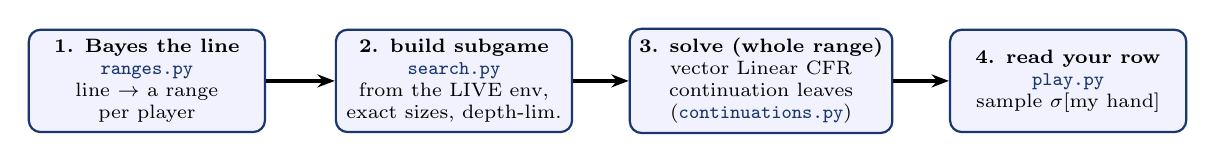
\begin{tikzpicture}[font=\scriptsize, >={Stealth[length=2.2mm]},
  s/.style={rectangle, rounded corners=1.5mm, draw=accent, fill=blue!5, thick,
            align=center, minimum height=13mm, minimum width=30mm}]
  \node[s] (a) at (0,0) {\textbf{1. Bayes the line}\\ \file{ranges.py}\\ line $\to$ a range\\ per player};
  \node[s] (b) at (3.9,0) {\textbf{2. build subgame}\\ \file{search.py}\\ from the LIVE env,\\ exact sizes, depth-lim.};
  \node[s] (c) at (7.8,0) {\textbf{3. solve (whole range)}\\ vector Linear CFR\\ continuation leaves\\ (\file{continuations.py})};
  \node[s] (d) at (11.7,0) {\textbf{4. read your row}\\ \file{play.py}\\ sample $\sigma$[my hand]};
  \draw[->, very thick] (a)--(b); \draw[->, very thick] (b)--(c); \draw[->, very thick] (c)--(d);
\end{tikzpicture}
\end{center}

\paragraph{Bayes ranges (\file{ranges.py}).} \fn{bayes\_ranges} replays the public
history under the blueprint: \texttt{range\_p[h] $\propto \prod$ $\sigma$(action $\mid$
infoset of $p$ holding $h$)}, card-removal masked. Hands that fit the line get
boosted; hands the blueprint would (almost) never play this way go to $\sim 0$.
(Validated: after an SB jam, the SB range puts $\sim 10^{3}\times$ more mass on AA
than on 72o.)

\paragraph{Trick 2 --- solve for the whole range (\file{search.py}).}
\fn{build\_engine\_subgame} enumerates the abstract betting tree \emph{from the
agent's live engine state} (so pot/stacks/exact sizes --- including an opponent's
off-tree size, already in the state --- are exact, no rounding) into a
\file{rebel\_py} \fn{Subgame}, which \fn{CfrSolver} solves over all 1326 hands at
once. The agent reads off the row of its actual hand only at the end
(\fn{\_root\_action\_probs}). On the river this is exact (true terminals, no
continuations): re-solving reaches \textbf{0.002 bb/hand} exploitability.

\paragraph{Trick 1 --- continuation strategies (\file{continuations.py}).} Before
the river, a leaf (the street boundary) is not the end of the hand, so its value
depends on how play continues. Valuing it with a single fixed continuation lets
the search above cheat. \fn{bias\_strategy} builds the 4 continuations
(blueprint, fold/call/raise-biased --- multiply one action family's probability by
a constant and renormalize, support preserved); the opponent's choice among them
is folded into the CFR solve at the leaf, so the equilibrium is robust to all
$4^{2}$ continuations.

\paragraph{Nested re-solving.} An opponent bet outside the agent's size grid is
already in the live engine state (applied exactly, via \texttt{step\_raise\_to}),
so re-solving \emph{from that state} prices the exact size with no rounding ---
just call \fn{resolve} again.

\begin{lstlisting}[style=py, caption={\file{play.py} --- the agent. Preflop (dense abstraction) plays the blueprint directly; on the river it re-solves the whole range and reads its row. Postflop search needs a postflop-trained blueprint to value continuation leaves.}]
def act(self, env):
    st = env.state()
    if int(st.street) not in self.search_streets:   # preflop / no postflop net
        return self.bp.sample(st, self.rng)          # blueprint, look at my cards
    probs, _, _ = resolve(env, self.bp, self.cfg)    # solve the WHOLE range
    h = hand_index(*my_hole_cards)
    return sample(probs[h])                          # my row, only at the end
\end{lstlisting}

% ════════════════════════════════════════════════════════════════════════════
\section{The cluster trainer (\file{blueprint\_mp.py})}
% ════════════════════════════════════════════════════════════════════════════

Tabular MCCFR is CPU/RAM-bound --- the 64-core, no-GPU profile Pluribus trained
on. \fn{train\_blueprint\_mp} is synchronous data-parallel CFR: each round ships
the master tables to $W$ workers; each worker deep-copies them, runs a batch of
traversals (adapting locally), and returns only its \textbf{increments}; the
master sums them. Because regret/strategy-sum are additive, summing $W$ workers'
increments $\approx$ doing $W\times$ the traversals of sequential CFR.

\begin{center}
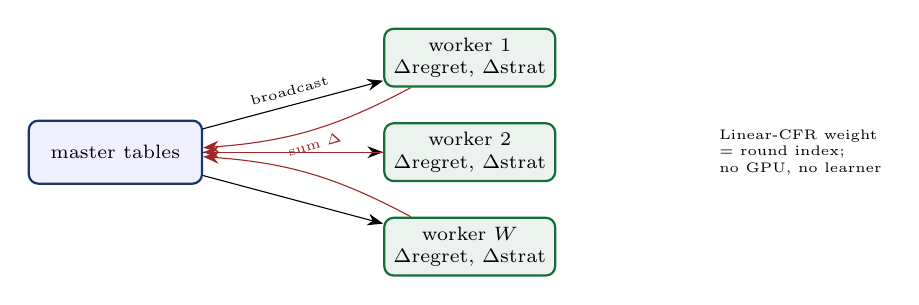
\begin{tikzpicture}[font=\scriptsize, >={Stealth[length=2mm]},
  m/.style={rectangle, rounded corners=1.2mm, draw=accent, fill=blue!6, thick, align=center, minimum height=8mm, minimum width=22mm},
  w/.style={rectangle, rounded corners=1.2mm, draw=heroG, fill=heroG!8, thick, align=center, minimum height=7mm, minimum width=20mm}]
  \node[m] (M) at (0,0) {master tables};
  \node[w] (w1) at (4.5,1.2) {worker 1\\ \scriptsize $\Delta$regret, $\Delta$strat};
  \node[w] (w2) at (4.5,0.0) {worker 2\\ \scriptsize $\Delta$regret, $\Delta$strat};
  \node[w] (w3) at (4.5,-1.2) {worker $W$\\ \scriptsize $\Delta$regret, $\Delta$strat};
  \draw[->] (M) -- node[above,sloped,font=\tiny]{broadcast} (w1);
  \draw[->] (M) -- (w2); \draw[->] (M) -- (w3);
  \draw[->, villR] (w1) to[bend left=12] node[below,sloped,font=\tiny]{sum $\Delta$} (M);
  \draw[->, villR] (w2) -- (M);
  \draw[->, villR] (w3) to[bend right=12] (M);
  \node[align=left, font=\tiny] at (8.7,0) {Linear-CFR weight\\ $=$ round index;\\ no GPU, no learner};
\end{tikzpicture}
\end{center}

\texttt{scripts/run\_pluribus\_cluster.sh} launches it inside the Singularity
image with \emph{no} \texttt{--nv} (the blueprint never touches CUDA). At
700\,GB-RAM / 64-core scale the keyspace would be \emph{sharded} across workers
(each owns a hash bucket, no per-round broadcast) --- the additive merge here is
the primitive that extension builds on.

% ════════════════════════════════════════════════════════════════════════════
\section{Correspondence at a glance, and what is validated}
% ════════════════════════════════════════════════════════════════════════════

\begin{center}\small
\begin{tabular}{@{}lll@{}}
\toprule
Pluribus idea (tutorial) & file $\cdot$ function & status \\
\midrule
information abstraction (k-means equity) & \file{abstraction}$\cdot$\fn{bucket\_cards} & impl.; postflop k-means not yet exercised \\
action abstraction (few bet sizes) & \file{abstraction}$\cdot$\fn{ActionAbstraction} & validated (pushfold gate) \\
Linear MCCFR, external sampling & \file{mccfr}$\cdot$\fn{traverse} & validated vs Nash oracle \\
blueprint $=$ avg strategy (tables) & \file{blueprint}$\cdot$\fn{Blueprint} & validated (push/fold) \\
Bayes the line $\to$ ranges & \file{ranges}$\cdot$\fn{bayes\_ranges} & validated (post-jam range) \\
Trick 1: continuation strategies & \file{continuations}$\cdot$\fn{bias\_strategy} & impl. + unit-tested \\
Trick 2: solve the whole range & \file{search}$\cdot$\fn{resolve} & validated (river $\to 0$) \\
nested re-solving (off-tree sizes) & \file{search} (live-state re-solve) & impl. \\
the play-time loop & \file{play}$\cdot$\fn{PluribusAgent} & impl. (river + preflop) \\
64-core blueprint, no GPU & \file{blueprint\_mp} & validated (parallel merge) \\
\bottomrule
\end{tabular}
\end{center}

\paragraph{Hard gates (run them).}
\begin{lstlisting}[style=py]
PYTHONPATH=engine/build:trainer python -m pluribus.validate            # both phases
PYTHONPATH=engine/build:trainer python trainer/tests/test_pluribus_phase1.py
PYTHONPATH=engine/build:trainer python trainer/tests/test_pluribus_phase2.py
\end{lstlisting}

Phase 1 (\fn{validate\_pushfold}) trains a 10bb push/fold blueprint and checks it
reproduces \texttt{evaluate.pushfold\_solver}'s Nash equilibrium (aggregate ranges
within $\sim 0.3$\%, decisive-hand misplay $< 3$\%). Phase 2
(\fn{validate\_river\_resolve}) re-solves several river spots over the whole
1326-hand range and asserts $< 0.05$ bb/hand exploitability (observed
$\sim 0.002$). The mixed-band frequency differences from the exact oracle are
expected sampling variance, not error (Pluribus's blueprint is itself a sampled
approximation; the real run uses far more iterations).

\paragraph{Out of scope (first pass).} A true 6-max engine (the engine is
heads-up; Pluribus's \emph{method} is what is ported); suit-isomorphism beyond
k-means; a C++ port for max throughput; cross-street continuation rollouts for
flop/turn search (the river re-solve and the continuation \emph{gadget} are
implemented; wiring a postflop-trained blueprint through the leaf rollout is the
documented next step); and a UI/Slumbot seat for the agent (the \file{play}
policy is designed to drop in, as the ReBeL net was).

\paragraph{An engine bug fixed along the way.} External-sampling MCCFR calls
\texttt{Env.clone()} once per branched action. \texttt{clone()} was constructing a
throwaway \texttt{Env} via the public constructor, which rebuilt the entire
\texttt{HandEvaluator} lookup table ($\approx 2$\,ms) only to discard it --- a
silent tax on \emph{all} CFR traversal in the repo (Deep CFR clones too). A
one-line private tag constructor that builds nothing dropped \texttt{clone()} from
$1950\,\mu s$ to $1.07\,\mu s$ ($\sim 1800\times$), turning the blueprint from
150 to 4500 iters/s.

\vspace{4mm}\hrule\vspace{2mm}
{\small \textbf{Paper.} Brown \& Sandholm, \emph{Superhuman AI for multiplayer
poker}, Science 365 (2019). \quad \textbf{Code.} \file{trainer/pluribus/} (+
\file{trainer/rebel\_py} for the shared search primitives).}

\end{document}
